\subsection{Simulation Results}
The simulation results for the $NO_x$ reduction prediction per time step for all the tests are plotted below.

\begin{figure}[H]
        \begin{minipage}{0.49\textwidth}
                \begin{figure}[H]
                        \centering
                        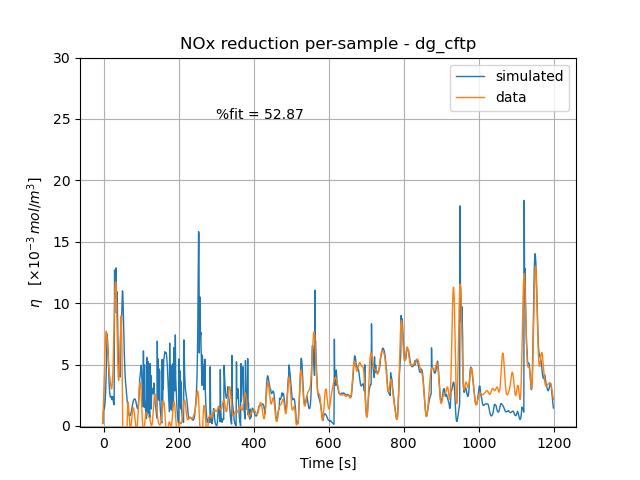
\includegraphics[width=\textwidth]{\froot/figs/15_figs/eta_sim_dg_cftp.png}
                \end{figure}
        \end{minipage}
        \begin{minipage}{0.49\textwidth}
                \begin{figure}[H]
                        \centering
                        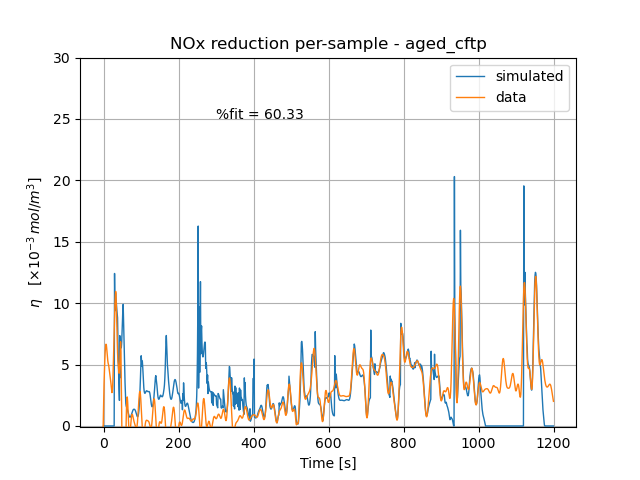
\includegraphics[width=\textwidth]{\froot/figs/15_figs/eta_sim_aged_cftp.png}
                \end{figure}
        \end{minipage}
        \caption{System response for cold FTP data}
\end{figure}

\begin{figure}[H]
        \begin{minipage}{0.49\textwidth}
                \begin{figure}[H]
                        \centering
                        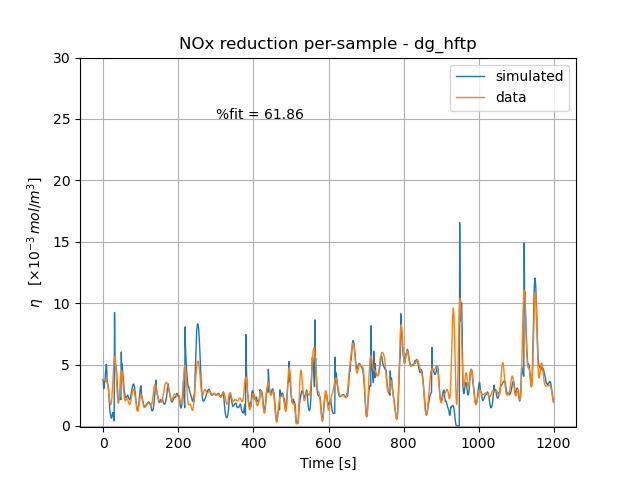
\includegraphics[width=\textwidth]{\froot/figs/15_figs/eta_sim_dg_hftp.png}
                \end{figure}
        \end{minipage}
        \begin{minipage}{0.49\textwidth}
                \begin{figure}[H]
                        \centering
                        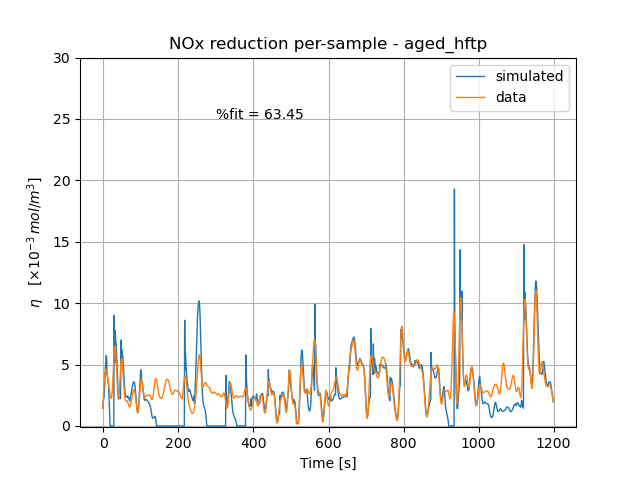
\includegraphics[width=\textwidth]{\froot/figs/15_figs/eta_sim_aged_hftp.png}
                \end{figure}
        \end{minipage}
        \caption{System response for hot FTP data}
\end{figure}

\begin{figure}[H]
        \begin{minipage}{0.49\textwidth}
                \begin{figure}[H]
                        \centering
                        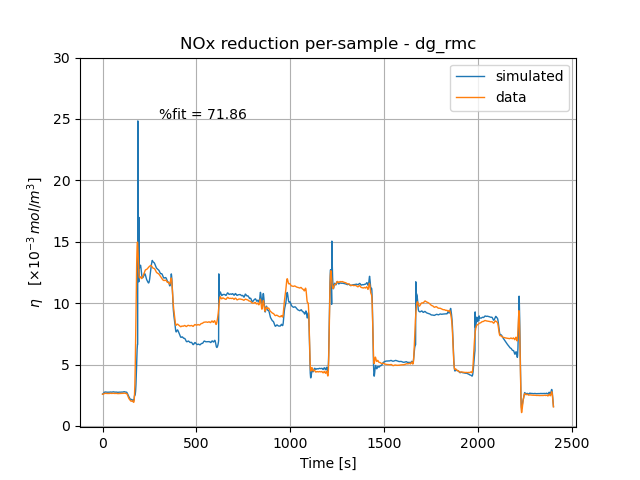
\includegraphics[width=\textwidth]{\froot/figs/15_figs/eta_sim_dg_rmc.png}
                \end{figure}
        \end{minipage}
        \begin{minipage}{0.49\textwidth}
                \begin{figure}[H]
                        \centering
                        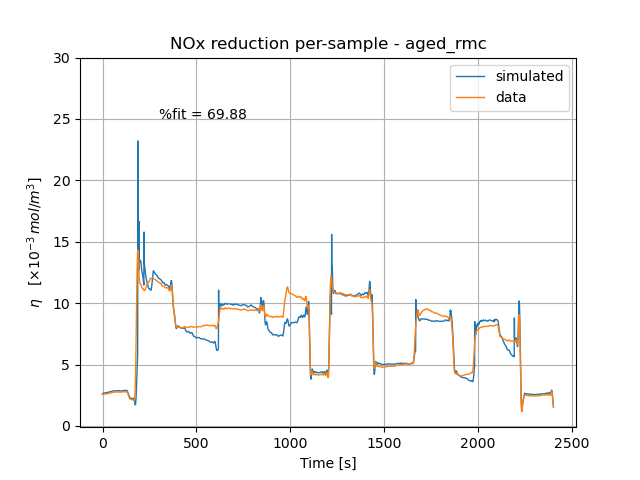
\includegraphics[width=\textwidth]{\froot/figs/15_figs/eta_sim_aged_rmc.png}
                \end{figure}
        \end{minipage}
        \caption{System response for RMC data}
\end{figure}


\begin{table}[H]
        \centering
        \caption{$\%$fit of the models with test data}
        \label{tab::results}
        \begin{tabular}{l l c c}
                \hline \hline
                Age & Test & Switched Nonlinear Model & Linearized CSTR Model \\ \hline \hline
                Degreened & RMC & 71.86 & 19.98 \\
                Aged      & RMC & 69.88 & 27.66 \\ \hline
                % =========================================
                Degreened & hot FTP & 61.86 & 7.10 \\
                Aged      & hot FTP & 63.45 & 7.38 \\ \hline
                % =========================================
                Degreened & Cold FTP & 52.87 & 23.24 \\
                Aged      & Cold FTP & 60.33 & 23.19 \\ \hline
                \hline
        \end{tabular}

        $\%fit = 100 \times \lr{1 - \frac{\norm{Y- \hat Y}}{\norm{Y -
        mean(Y)}}}$ \\
        $\%fit$ is the percentage of the measured output that was explained by the
        model.
\end{table}

Thus, the switched nonlinear model consistently fits the data with a goodness of fit value greater than $50\%$ for all
the test-cases. While the linearized CSTR model, though identifiable, has no further room for improvement in terms of
model refinement, the proposed hybrid nonlinear model has further potential for refinement resulting in lower prediction
errors than presented. Specifically, further work needs to be done in the development of appropriate switching
conditions between the saturated and desaturated models. Moreover, the model offers the flexibility of incorporating
more complex models of underlying physical properties (rate-constants, residence time, etc.) relaxing or reworking the
assumptions to better fit the operating conditions.
